\begin{figure*}
\centering
\begin{subfigure}[t]{0.475\textwidth}
\begin{tikzpicture}[thick, scale=0.7, every label/.style={align=left, scale=0.7}]
   \pie[text=legend, hide number, color={blue!60, cyan!60, yellow!60}]{
      32.6/32.6\%,
      55.8/55.8\%,
      11.6/11.6\%
}
\end{tikzpicture}
\caption{Discrepancies from standards.}
\label{fig:stdDiscrepSources}
\end{subfigure}
\hfill
\begin{subfigure}[t]{0.475\textwidth}
\begin{tikzpicture}[thick, scale=0.7, every label/.style={align=left, scale=0.7}]
   \pie[text=legend, hide number, color={blue!60, yellow!60, orange!60}]{
      16.1/16.1\%,
      64.5/64.5\%,
      19.4/19.4\%
}
\end{tikzpicture}
\caption{Discrepancies from ``meta-level'' sources.}
\label{fig:metaDiscrepSources}
\end{subfigure}
\vskip\baselineskip
\begin{subfigure}[t]{0.475\textwidth}
\begin{tikzpicture}[thick, scale=0.7, every label/.style={align=left, scale=0.7}]
   \pie[text=legend, hide number, color={blue!60, yellow!60, orange!60}]{
      45.5/45.5\%,
      36.4/36.4\%,
      18.2/18.2\%
}
\end{tikzpicture}
\caption{Discrepancies from textbooks.}
\label{fig:textDiscrepSources}
\end{subfigure}
\hfill
\begin{subfigure}[t]{0.475\textwidth}
\begin{tikzpicture}[thick, scale=0.7, every label/.style={align=left, scale=0.7}]
   \pie[text=legend, hide number, color={blue!60, yellow!60, orange!60, red!60, blue!60!cyan!60}]{
      12.1/12.1\%,
      48.5/48.5\%,
      27.3/27.3\%,
      3.0/3.0\%,
      9.1/9.1\%
}
\end{tikzpicture}
\caption{Discrepancies from other sources.}
\label{fig:otherDiscrepSources}
\end{subfigure}
\vskip\baselineskip
\begin{subfigure}[t]{0.475\textwidth}
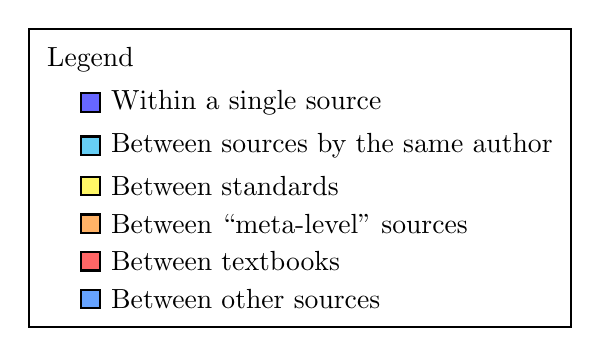
\begin{tikzpicture}
\matrix [thick, draw=black] {
\node[label={[centered]:Legend}] {{}}; \\
\node[thick, shape=rectangle, draw=black, fill=blue!60, label=right:{Within a single source}](0) {}; \\
\node[thick, shape=rectangle, draw=black, fill=cyan!60, label=right:{Between sources by the same author}](1) {}; \\
\node[thick, shape=rectangle, draw=black, fill=yellow!60, label=right:{Between standards}](2) {}; \\
\node[thick, shape=rectangle, draw=black, fill=orange!60, label=right:{Between ``meta-level'' sources}](3) {}; \\
\node[thick, shape=rectangle, draw=black, fill=red!60, label=right:{Between textbooks}](4) {}; \\
\node[thick, shape=rectangle, draw=black, fill=blue!60!cyan!60, label=right:{Between other sources}](5) {}; \\
};
\end{tikzpicture}
\end{subfigure}
\hfill
\caption{Sources of discrepancies based on \hyperref[sources]{source category}.}
\label{fig:discrepSources}
\end{figure*}
